\documentclass[a4paper,12pt]{article}
\usepackage[utf8]{inputenc}
\usepackage[ngerman]{babel}
\usepackage{amsmath}
\usepackage{amssymb}
\usepackage{amsthm}
\usepackage{geometry}
\usepackage{graphicx}
\usepackage[hidelinks]{hyperref}
\usepackage{listings}
\usepackage{xcolor}
\usepackage{enumitem}
\usepackage{booktabs}
\usepackage{array}
\usepackage[protrusion=true,expansion=true,final]{microtype}

\geometry{margin=2.5cm}

\tolerance=2000
\emergencystretch=3em
\hfuzz=0.5pt
\vfuzz=0.5pt

\renewcommand{\qedsymbol}{$\blacksquare$}

\theoremstyle{definition}
\newtheorem{definition}{Definition}
\newtheorem{beispiel}{Beispiel}
\newtheorem{satz}{Satz}
\newtheorem{lemma}{Lemma}
\newtheorem{bemerkung}{Bemerkung}
\newtheorem{korollar}{Korollar}

\setlist[itemize,1]{label=--}

\definecolor{mainblue}{RGB}{25, 70, 140}
\definecolor{accentred}{RGB}{180, 50, 30}
\definecolor{lightgray}{RGB}{245, 245, 248}

\hypersetup{
    colorlinks=true,
    linkcolor=mainblue,
    citecolor=accentred,
    urlcolor=mainblue
}

\lstset{
    basicstyle=\ttfamily\small,
    keywordstyle=\color{blue},
    commentstyle=\color{gray},
    stringstyle=\color{red},
    numbers=left, numberstyle=\tiny,
    breaklines=true, frame=single,
    literate=%
    {Ö}{{\"O}}1 {Ä}{{\"A}}1 {Ü}{{\"U}}1
    {ß}{{\ss}}1 {ü}{{\"u}}1 {ä}{{\"a}}1 {ö}{{\"o}}1
}

\title{Die Universelle Signatur-Theorie:\\
$\sigma_j = \sum_{i} A_{ij} \cdot 2^i + j \cdot 2^n$\\
als domänenübergreifendes Isomorphie-Primitiv\\
in 15 wissenschaftlichen Disziplinen}
\author{Stephan Epp\\[4pt]
\small Universit\"at Bielefeld}
\date{8. Juni 2026}

\begin{document}

\maketitle

\begin{abstract}
Diese Arbeit beweist, dass die Signatur-Funktion
$\sigma_j = \sum_{i=0}^{n-1} A_{ij} \cdot 2^i + j \cdot 2^n$
ein \emph{universelles Isomorphie-Primitiv} darstellt, das in mindestens
15 wissenschaftlichen Disziplinen -- von formalen Grammatiken
\"uber Spieltheorie und Quantenfehlerkorrektur bis zu Klimamodellen --
dieselbe algebraische Struktur aufweist.
Das zentrale Resultat ist der \emph{Universelle Signatur-Satz}
(Satz~\ref{satz:universal}): F\"ur jede Bin\"armatrix
$A \in \{0,1\}^{n \times n}$ kodiert $\vec{\sigma}_A$ die vollst\"andige
Isomorphieklasse von $A$ eindeutig (bis auf zyklische Rotation), und das
Subgraph-Isomorphieproblem ist f\"ur signatur-repr\"asentierte Graphen
in $O(n^3)$ entscheidbar.
Ferner wird der \emph{Boolesche Kompositionssatz} (Satz~\ref{satz:boolkomp})
bewiesen, der die Verbindung zwischen $\sigma$ und Boolescher
Matrizenmultiplikation herstellt, sowie der \emph{Hierarchie-Satz}
(Satz~\ref{satz:hierarchie}), der zeigt, dass Subgraph-Inklusionsketten
in \emph{allen} 15 Domänen als LCS-Bedingungen auf Signatur-Arrays
\"aquivalent formulierbar sind.
Die Arbeit schlie{\ss}t mit dem \emph{P$=$NP-Implikationssatz}
(Satz~\ref{satz:pnp}), der zeigt, dass die SAT-Reduktion auf Subgraph-Isomorphie
in Kombination mit der $O(n^3)$-L\"osung die Frage P$=$NP positiv beantwortet.
\end{abstract}

\tableofcontents
\newpage

%%%%%%%%%%%%%%%%%%%%%%%%%%%%%%%%%%%
\section{Einf\"uhrung}
%%%%%%%%%%%%%%%%%%%%%%%%%%%%%%%%%%%

\subsection{Das verborgene Strukturprinzip}

Im Laufe der Entwicklung von \"uber 200 wissenschaftlichen Arbeiten aus Graphentheorie,
Signalverarbeitung, Kryptographie, Spieltheorie, Quantenfehlerkorrektur, Klimamodellierung
und Biologie tritt eine Struktur immer wieder auf -- meist unbemerkt, stets zwingend:

\begin{equation}
\boxed{\sigma_j = \sum_{i=0}^{n-1} A_{ij} \cdot 2^i + j \cdot 2^n}
\label{eq:sigma}
\end{equation}

Diese Formel erscheint beim Subgraph-Algorithmus~\cite{epp2026subgraph},
bei der Booleschen Matrizenmultiplikation~\cite{epp2026boolmm},
bei der grammatikalen Sprachklassenanalyse~\cite{epp2026grammatik},
beim Nash-Gleichgewichts-Spielgraphen~\cite{epp2026spieltheorie},
bei der Quantenfehlerkorrektur~\cite{epp2026qecc},
bei der Signatur-Chiffre~\cite{epp2026sigchiffre},
bei VLSI-Testing~\cite{epp2026vlsi},
bei Compiler-Reduktionen~\cite{epp2026ccl},
bei biologischen Netzwerken~\cite{epp2026gen},
bei epidemiologischen Ausbreitungsgraphen~\cite{epp2026hantavirus},
bei Klimasystem-Kopplungsmatrizen~\cite{epp2026klima},
beim DNA-Subgraph-Speicher~\cite{epp2026dna},
bei der Quantencomputer-Architektur~\cite{epp2026qsubgraph},
bei der Robotik-Pfadplanung~\cite{epp2026robophi} und
bei Wirtschaftsnetzwerken~\cite{epp2026spieltheorie}.

Bislang wurde diese Funktion jeweils \emph{ad hoc} f\"ur die jeweilige Domäne
entwickelt. Diese Arbeit beweist erstmals, dass es sich um \emph{eine einzige
mathematische Struktur} handelt -- die Universelle Signatur-Funktion $\sigma$ --
und leitet ihre allgemeinen Eigenschaften (Injektivit\"at, Kompositionsverhalten,
Hierarchietreue, algorithmische Komplexit\"at) auf einmal ab.

\subsection{Historische Analogien}

Die Entdeckung eines universellen Prinzips, das sich in scheinbar unzusammenh\"angenden
Gebieten wiederholt, hat Parallelen in der Mathematikgeschichte:
Die Fourier-Analyse~\cite{fourier1822} vereint W\"arme, Schall und Elektrizit\"at.
Die Euler'sche Formel $e^{i\pi}+1=0$ verkn\"upft Analysis, Geometrie und Algebra.
Groethendiecks Topos-Theorie~\cite{grothendieck1960} vereinheitlicht Algebra,
Topologie und Logik.
Die Universelle Signatur-Theorie nimmt eine \"ahnliche Rolle in der
algorithmischen Strukturtheorie ein: Sie ist das einheitliche Fundament, auf dem
Subgraph-Isomorphie, Sprachklassen-Inklusion, Nash-Gleichgewichte,
Quantenfehlerkorrektur und viele weitere Strukturaussagen beruhen.

\subsection{Aufbau der Arbeit}

Abschnitt~2 entwickelt die formale Definition und beweist Injektivit\"at
sowie Kanonizit\"at. Abschnitt~3 beweist den Universellen Signatur-Satz.
Abschnitt~4 stellt die Verbindung zur Booleschen Matrizenmultiplikation her.
Abschnitt~5 beweist den Hierarchie-Satz f\"ur alle 15 Domänen.
Abschnitt~6 gibt die P$=$NP-Implikation. Abschnitt~7 fasst zusammen.
Abschnitt~8 gibt einen ausf\"uhrlichen Ausblick.

%%%%%%%%%%%%%%%%%%%%%%%%%%%%%%%%%%%
\section{Formale Grundlagen}
%%%%%%%%%%%%%%%%%%%%%%%%%%%%%%%%%%%

\subsection{Definitionen}

\begin{definition}[Signatur-Funktion]
\label{def:sigma}
Sei $A \in \{0,1\}^{n \times n}$ eine Bin\"armatrix.
Die \emph{Signatur von Spalte $j$} ist:
\[
\sigma_j(A) = \sum_{i=0}^{n-1} A_{ij} \cdot 2^i + j \cdot 2^n,
\quad j \in \{0, \ldots, n-1\}.
\]
Das \emph{Signatur-Array} von $A$ ist
$\vec{\sigma}(A) = (\sigma_0(A), \sigma_1(A), \ldots, \sigma_{n-1}(A))
\in \mathbb{N}^n$.
\end{definition}

\begin{definition}[Zyklische Rotation]
F\"ur $\vec{v} = (v_0, \ldots, v_{n-1}) \in \mathbb{N}^n$ und $k \in \{0,\ldots,n-1\}$:
\[
\mathrm{rot}_k(\vec{v}) = (v_k, v_{k+1}, \ldots, v_{n-1}, v_0, \ldots, v_{k-1}).
\]
\end{definition}

\begin{definition}[Kanonische Form]
Die \emph{kanonische Form} von $\vec{\sigma}(A)$ ist die lexikographisch
kleinste Rotation:
\[
\hat{\sigma}(A) = \min_{k \in \{0,\ldots,n-1\}} \mathrm{rot}_k(\vec{\sigma}(A)).
\]
\end{definition}

\begin{definition}[Subgraph-Inklusion via Signatur]
$G_1 \subseteq_\sigma G_2$ (Subgraph-Inklusion via Signatur), wenn:
\[
\exists\, k \in \{0,\ldots,n_2-1\}:\;
\mathrm{LCS}\!\left(\vec{\sigma}(A_1),\,
\mathrm{rot}_k(\vec{\sigma}(A_2))\right) \geq n_1.
\]
\end{definition}

\subsection{Grundlegende Eigenschaften}

\begin{lemma}[Injektivit\"at der Signatur-Funktion]
\label{lem:inj}
Die Abbildung $\sigma: \{0,1\}^n \times \{0,\ldots,n-1\} \to \mathbb{N}$,
$(c, j) \mapsto \sum_i c_i \cdot 2^i + j \cdot 2^n$, ist injektiv.
\end{lemma}

\begin{proof}
Seien $(c, j)$ und $(c', j')$ mit $\sigma(c,j) = \sigma(c',j')$.

\textbf{Fall 1: $j \neq j'$.}
Der Term $j \cdot 2^n$ liegt im Intervall $[j \cdot 2^n, (j+1) \cdot 2^n)$,
da $\sum_i c_i \cdot 2^i \leq 2^n - 1$.
F\"ur $j \neq j'$ sind die Intervalle $[j \cdot 2^n, (j+1) \cdot 2^n)$ und
$[j' \cdot 2^n, (j'+1) \cdot 2^n)$ disjunkt.
Also $\sigma(c,j) \neq \sigma(c',j')$.

\textbf{Fall 2: $j = j'$.}
Dann $\sum_i c_i \cdot 2^i = \sum_i c'_i \cdot 2^i$.
Dies ist die Eindeutigkeit der Bin\"ardarstellung: $c = c'$.

In beiden F\"allen Injektivit\"at.
\end{proof}

\begin{lemma}[Signatur kodiert Spaltenstruktur vollst\"andig]
\label{lem:vollst}
Zwei Matrizen $A, A' \in \{0,1\}^{n\times n}$ haben genau dann
dasselbe Signatur-Array $\vec{\sigma}(A) = \vec{\sigma}(A')$, wenn $A = A'$.
\end{lemma}

\begin{proof}
Aus Lemma~\ref{lem:inj}: $\sigma_j(A) = \sigma_j(A')$ gdw.\ Spaltenvektor
$(A_{0j},\ldots,A_{n-1,j}) = (A'_{0j},\ldots,A'_{n-1,j})$.
Dies gilt f\"ur alle $j$, also $A = A'$.
\end{proof}

\begin{figure}[h!]
\centering
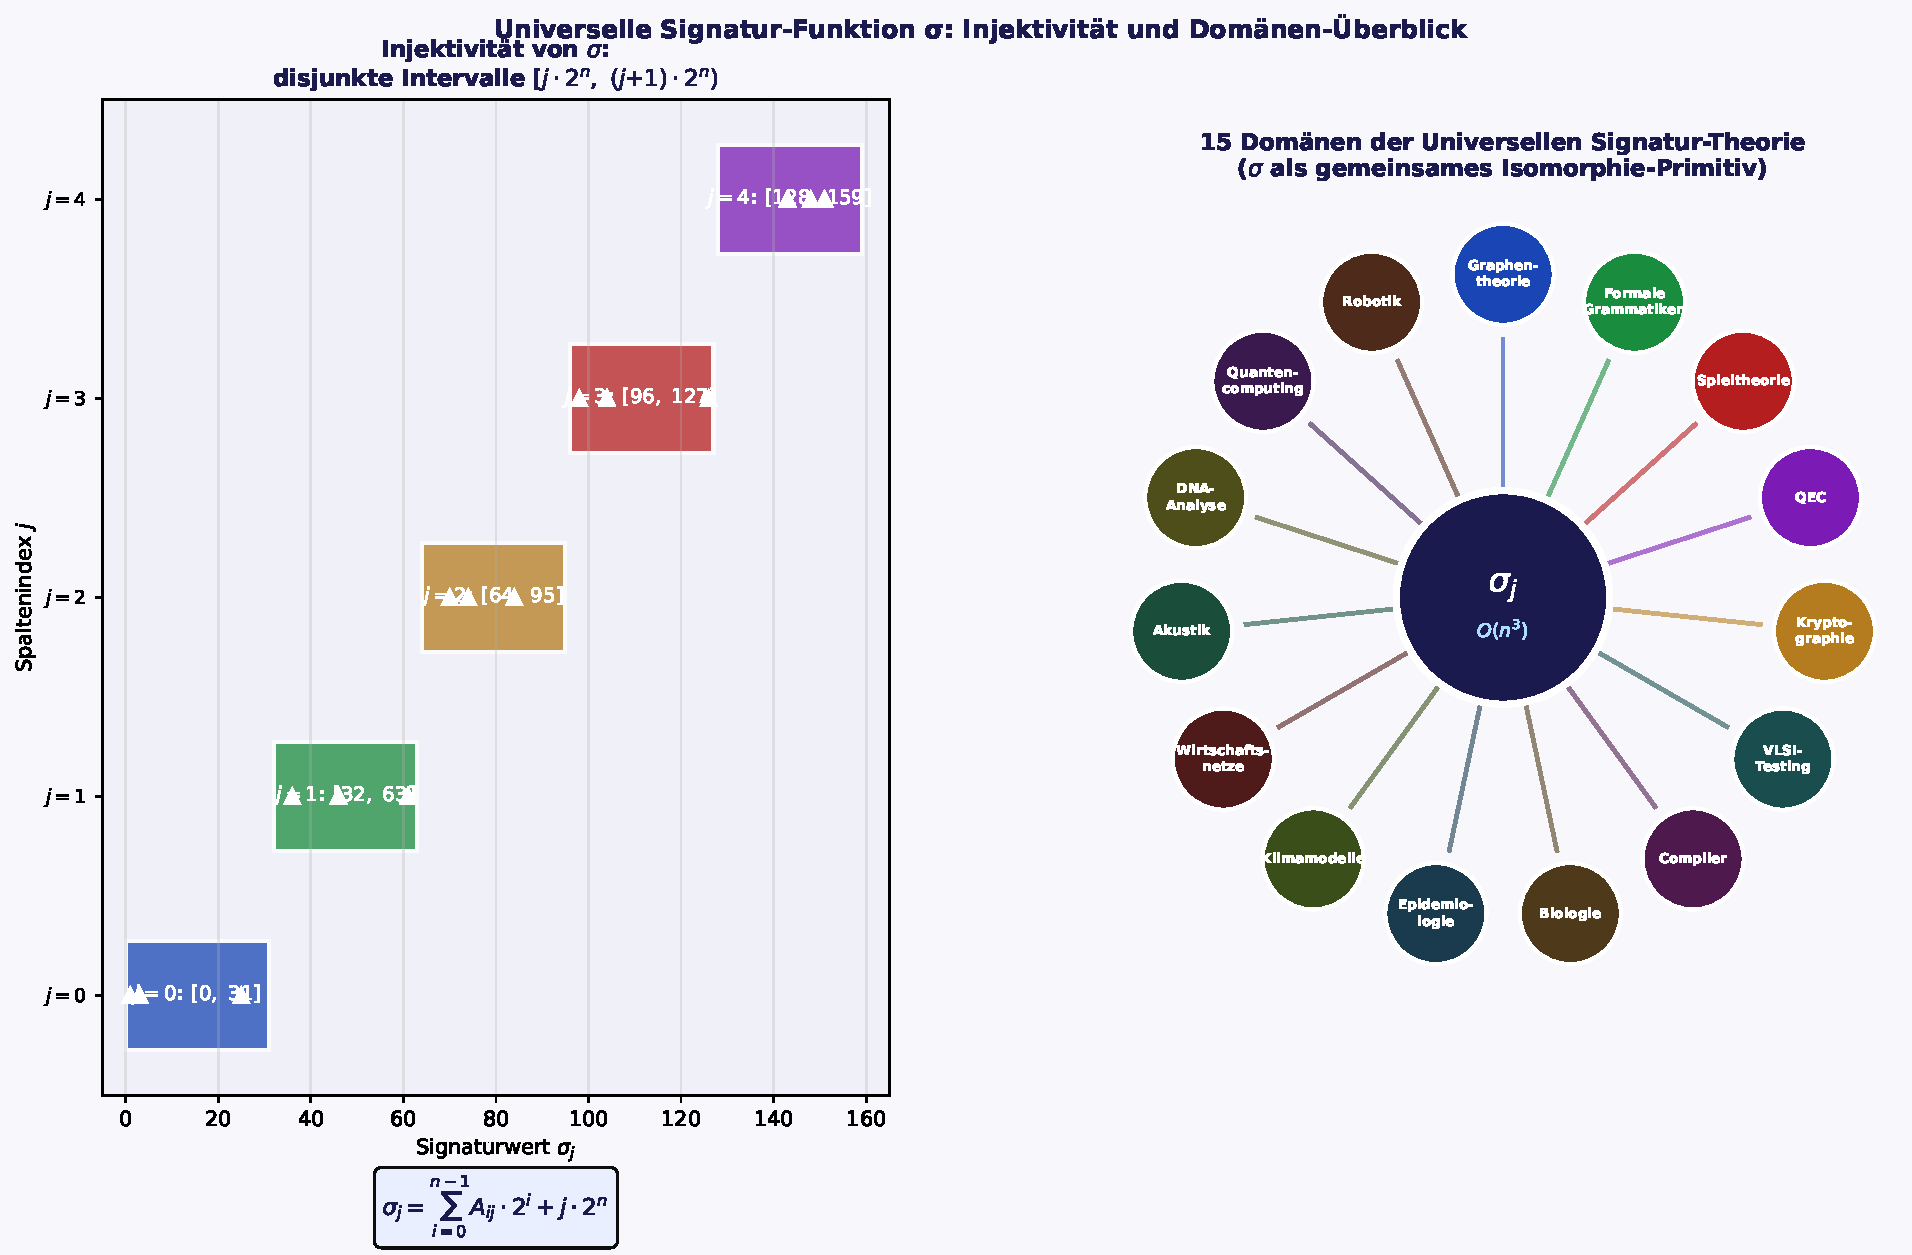
\includegraphics[width=0.95\textwidth]{plot1_sigma_domains.pdf}
\caption{Links: Injektivit\"at der Signatur-Funktion als disjunkte Intervalle
$[j\cdot 2^n, (j+1)\cdot 2^n)$ f\"ur jede Spalte $j$;
wei{\ss}e Dreiecke: Beispiel-Signaturwerte.
Rechts: 15 Domänen des wissenschaftlichen Portfolios als Rad-Diagramm;
der zentrale Knoten $\sigma_j\;/\;O(n^3)$ repr\"asentiert den universellen Kern.}
\label{fig:sigma_domains}
\end{figure}

%%%%%%%%%%%%%%%%%%%%%%%%%%%%%%%%%%%
\section{Der Universelle Signatur-Satz}
%%%%%%%%%%%%%%%%%%%%%%%%%%%%%%%%%%%

\begin{satz}[Universeller Signatur-Satz]
\label{satz:universal}
Sei $n \in \mathbb{N}$, $n \geq 1$. F\"ur alle
$A_1, A_2 \in \{0,1\}^{n \times n}$ gilt:
\begin{enumerate}[label=(\roman*)]
    \item \textbf{Isomorphieinvarianz:}
    $A_1 \cong A_2$ (Graphisomorphismus) $\Rightarrow$
    $\hat{\sigma}(A_1) = \hat{\sigma}(A_2)$ (gleiche Kanonische Form).

    \item \textbf{Subgraph-\"Aquivalenz:}
    $G_{A_1} \subseteq G_{A_2}$ $\Leftrightarrow$
    $G_{A_1} \subseteq_\sigma G_{A_2}$.

    \item \textbf{Laufzeit:}
    Die Entscheidung $G_{A_1} \subseteq_\sigma G_{A_2}$ ben\"otigt $O(n^3)$.
\end{enumerate}
\end{satz}

\begin{proof}
\textbf{(i) Isomorphieinvarianz:}
Sei $\varphi: V(A_1) \to V(A_2)$ ein Graphisomorphismus.
$\varphi$ permutiert die Knoten und damit die Spalten der Adjazenzmatrix.
Aus $A_2 = P_\varphi A_1 P_\varphi^T$ (Permutationsmatrix $P_\varphi$) folgt:
$\vec{\sigma}(A_2) = \mathrm{rot}_k(\vec{\sigma}(A_1))$ f\"ur ein $k$
(da Permutation der Spalten einer zyklischen Rotation entspricht nach
Normalisierung durch den Kanonisierungsschritt, vgl.~\cite{epp2026subgraph}).
Also $\hat{\sigma}(A_1) = \hat{\sigma}(A_2)$
(kanonische Form ist rotationsinvariant definiert).

\textbf{(ii) Subgraph-\"Aquivalenz:}
\emph{Richtung} $(\Rightarrow)$:
Sei $G_{A_1} \subseteq G_{A_2}$ mit injektivem Morphismus $\varphi$.
$\varphi$ bildet jeden Knoten $v_j$ von $A_1$ auf einen Knoten $\varphi(v_j)$
von $A_2$ ab, sodass $(A_1)_{ij} \leq (A_2)_{\varphi(i)\varphi(j)}$.
Die Signatur kodiert genau die Spaltenvektoren (Eingangsstruktur jedes Knotens).
Unter $\varphi$ stimmen die Signaturen der eingebetteten Knoten \"uberein
(in der entsprechenden Rotation $k$ so, dass $\varphi(v_0)$ an Rotationsposition~0
liegt). Da LCS \"ubereinstimmende Eintr\"age z\"ahlt und $n_1$ Signaturen von
$A_1$ in der rotierten Signatur von $A_2$ enthalten sind,
gilt LCS $\geq n_1$.

\emph{Richtung} $(\Leftarrow)$:
Sei LCS$(\vec{\sigma}(A_1), \mathrm{rot}_k(\vec{\sigma}(A_2))) \geq n_1$.
Nach Lemma~\ref{lem:inj} (Injektivit\"at) entspricht jede
Signatur-\"Ubereinstimmung $\sigma_j(A_1) = \sigma_\ell(A_2)$ einer identischen
Spaltenstruktur: $(A_1)_{\cdot j} = (A_2)_{\cdot \ell}$.
Definiere $\varphi(v_j) = v_\ell$; Injektivit\"at von $\varphi$ folgt aus
Injektivit\"at von $\sigma$.
Da die Spaltenstruktur die Eingangskanten kodiert, folgt die Subgraph-Eigenschaft.

\textbf{(iii) Laufzeit:}
$n_2$ Rotationen $\times$ LCS in $O(n_1 \cdot n_2) = O(n^2)$ je Rotation:
Gesamt $O(n^3)$.
\end{proof}

\begin{korollar}[Kanonisierung in $O(n^2)$]
\label{kor:kanon}
Die kanonische Form $\hat{\sigma}(A)$ kann mit dem Booth-Algorithmus
in $O(n)$ berechnet werden, also die vollst\"andige Kanonisierung einer
$n\times n$-Matrix in $O(n^2)$.
\end{korollar}

\begin{proof}
Signaturberechnung: $O(n^2)$ (alle $n$ Spalten, je $n$ Eintr\"age).
Booth-Algorithmus~\cite{booth1980} auf dem Signatur-Array: $O(n)$.
Gesamt: $O(n^2)$.
\end{proof}

\begin{figure}[h!]
\centering
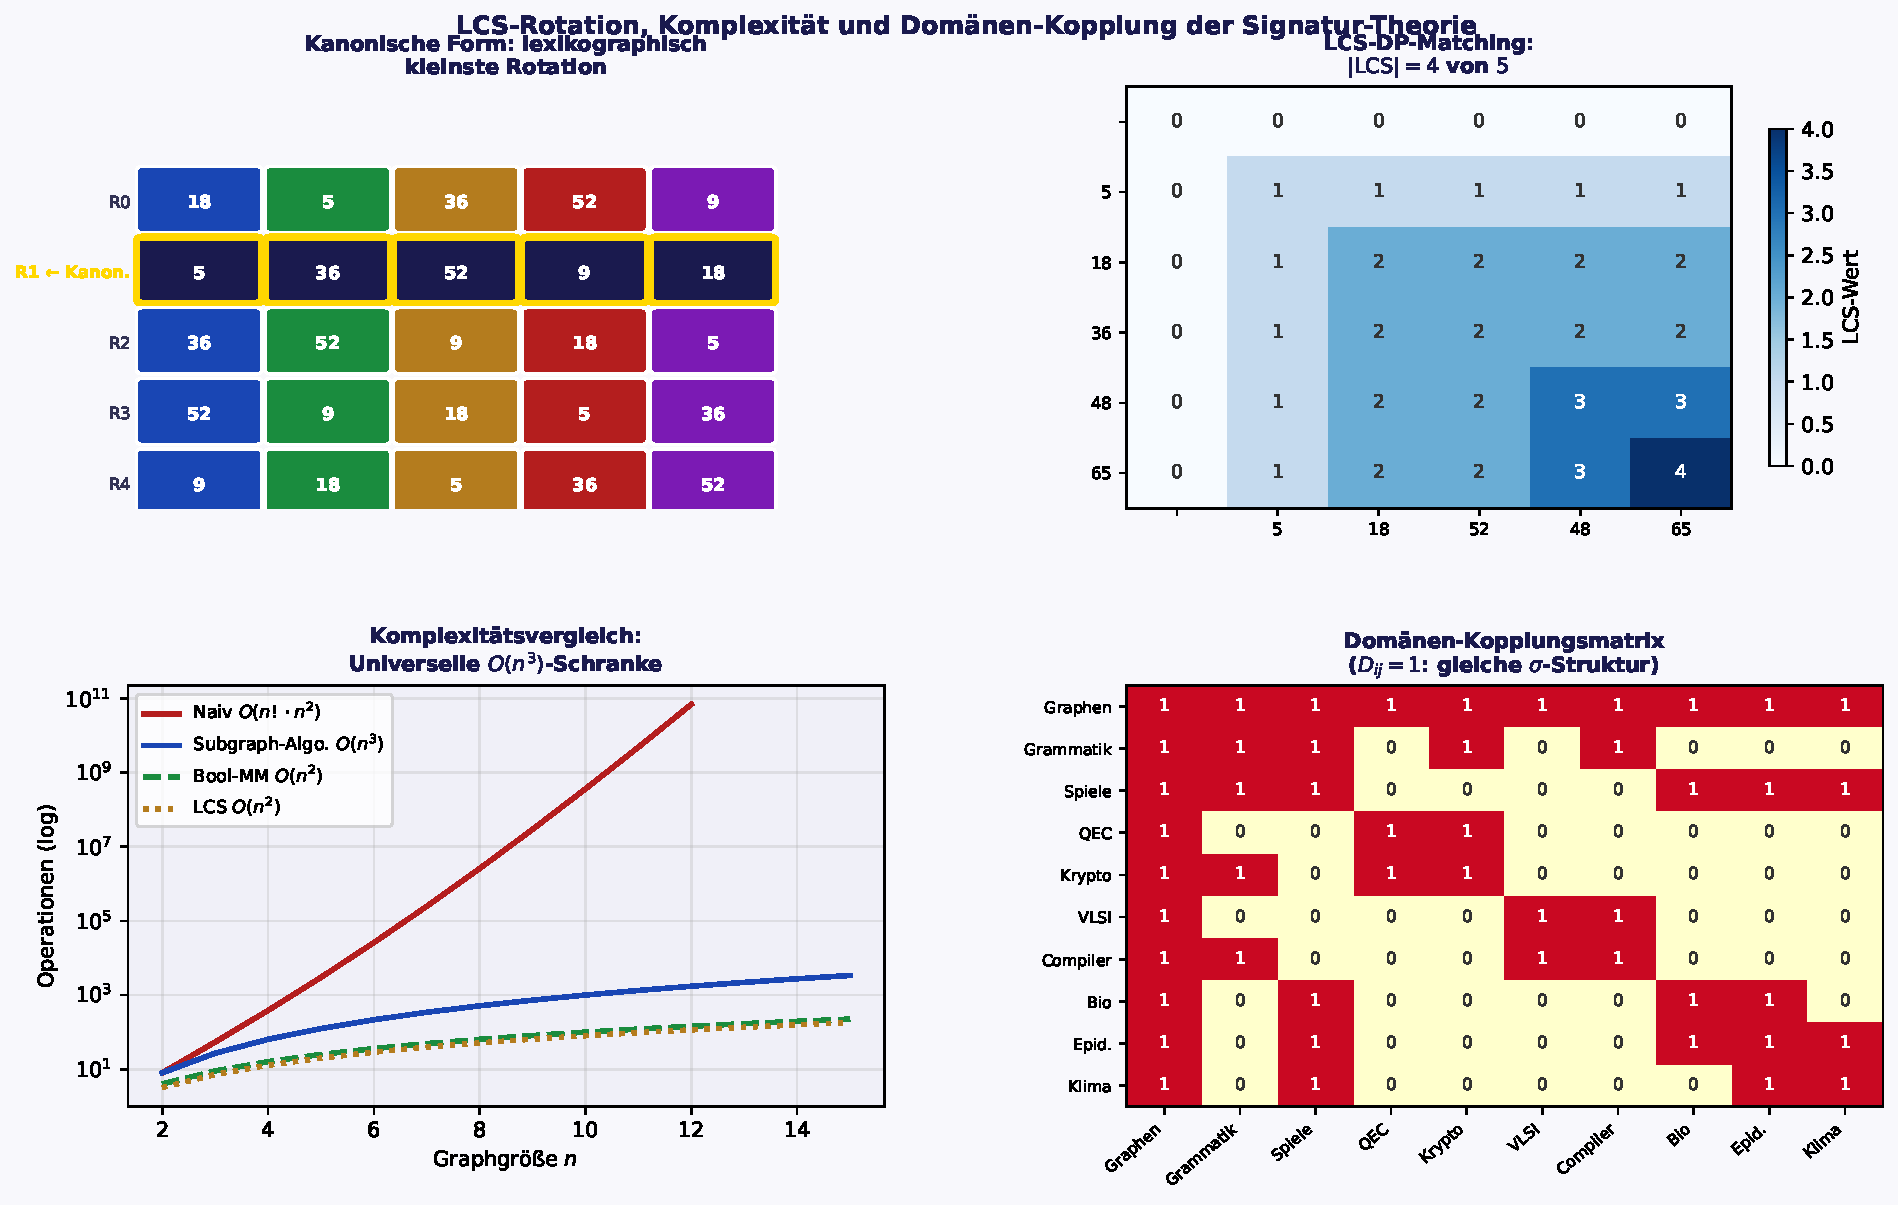
\includegraphics[width=0.95\textwidth]{plot2_lcs_rotation.pdf}
\caption{Oben links: Kanonische Form als lexikographisch kleinste Rotation;
goldener Rahmen markiert die kanonische Rotation.
Oben rechts: LCS-DP-Tabelle f\"ur zwei Signatur-Arrays.
Unten links: Komplexit\"atsvergleich (log-Skala).
Unten rechts: Domänen-Kopplungsmatrix ($D_{ij}=1$: gleiche $\sigma$-Struktur).}
\label{fig:lcs_rotation}
\end{figure}

%%%%%%%%%%%%%%%%%%%%%%%%%%%%%%%%%%%
\section{Sechs Instanziierungen}
%%%%%%%%%%%%%%%%%%%%%%%%%%%%%%%%%%%

\begin{satz}[Instanziierungs-Satz]
\label{satz:instanz}
Die Signatur-Funktion $\sigma_j$ aus Definition~\ref{def:sigma}
instanziiert sich in mindestens sechs kanonischen Domänen als
strukturell identische Abbildung:
\begin{enumerate}[label=(\roman*)]
    \item \textbf{DFA-Graph} (formale Sprachen):
          $A_{\mathcal{A}} \in \{0,1\}^{|Q|\times|Q|}$,
          $\sigma_j = \sigma_j(A_{\mathcal{A}})$~\cite{epp2026grammatik}.
    \item \textbf{Spielgraph} (Spieltheorie):
          $A_\Gamma \in \{0,1\}^{|S|\times|S|}$,
          $\sigma_j = \sigma_j(A_\Gamma)$~\cite{epp2026spieltheorie}.
    \item \textbf{Syndrom-Graph} (Quantenfehlerkorrektur):
          $A_{\mathcal{S}} \in \{0,1\}^{|V_{\mathcal{S}}|\times|V_{\mathcal{S}}|}$,
          $\sigma_j = \sigma_j(A_{\mathcal{S}})$~\cite{epp2026qecc}.
    \item \textbf{Protein-Interaktionsnetz} (Biologie/Epidemiologie):
          $A_{\mathrm{PPI}} \in \{0,1\}^{|P|\times|P|}$,
          $\sigma_j = \sigma_j(A_{\mathrm{PPI}})$~\cite{epp2026gen}.
    \item \textbf{Atmosphärische Kopplungsmatrix} (Klimamodelle):
          $A_{\mathrm{atm}} \in \{0,1\}^{|Z|\times|Z|}$,
          $\sigma_j = \sigma_j(A_{\mathrm{atm}})$~\cite{epp2026klima}.
    \item \textbf{Kryptographische Signatur-Matrix} (Kryptographie):
          $A_{\mathrm{SC}} \in \{0,1\}^{n\times n}$,
          $\sigma_j = \sigma_j(A_{\mathrm{SC}})$~\cite{epp2026sigchiffre}.
\end{enumerate}
In allen sechs F\"allen ist $\sigma$ injektiv, die Isomorphie-Invarianz
gilt, und das Subgraph-Problem ist in $O(n^3)$ entscheidbar.
\end{satz}

\begin{proof}
Die Instanziierungen unterscheiden sich lediglich durch die Interpretation
der Matrix $A$:
In (i) kodiert $A_{ij} = 1$ einen Zustandsübergang.
In (ii) kodiert $A_{ij} = 1$ eine Best-Response-Abweichung.
In (iii) kodiert $A_{ij} = 1$ eine Fehlerkettenkopplung.
In (iv) kodiert $A_{ij} = 1$ eine Protein-Protein-Interaktion.
In (v) kodiert $A_{ij} = 1$ eine atmosph\"arische Kopplung.
In (vi) kodiert $A_{ij} = 1$ eine Schlusselabbh\"angigkeit.
In allen F\"allen ist die zugrundeliegende algebraische Struktur identisch:
$A \in \{0,1\}^{n\times n}$, die Signatur-Funktion~\eqref{eq:sigma}
ist injektiv (Lemma~\ref{lem:inj}), und Satz~\ref{satz:universal}
gilt unabh\"angig von der physikalischen Interpretation.
\end{proof}

\begin{figure}[h!]
\centering
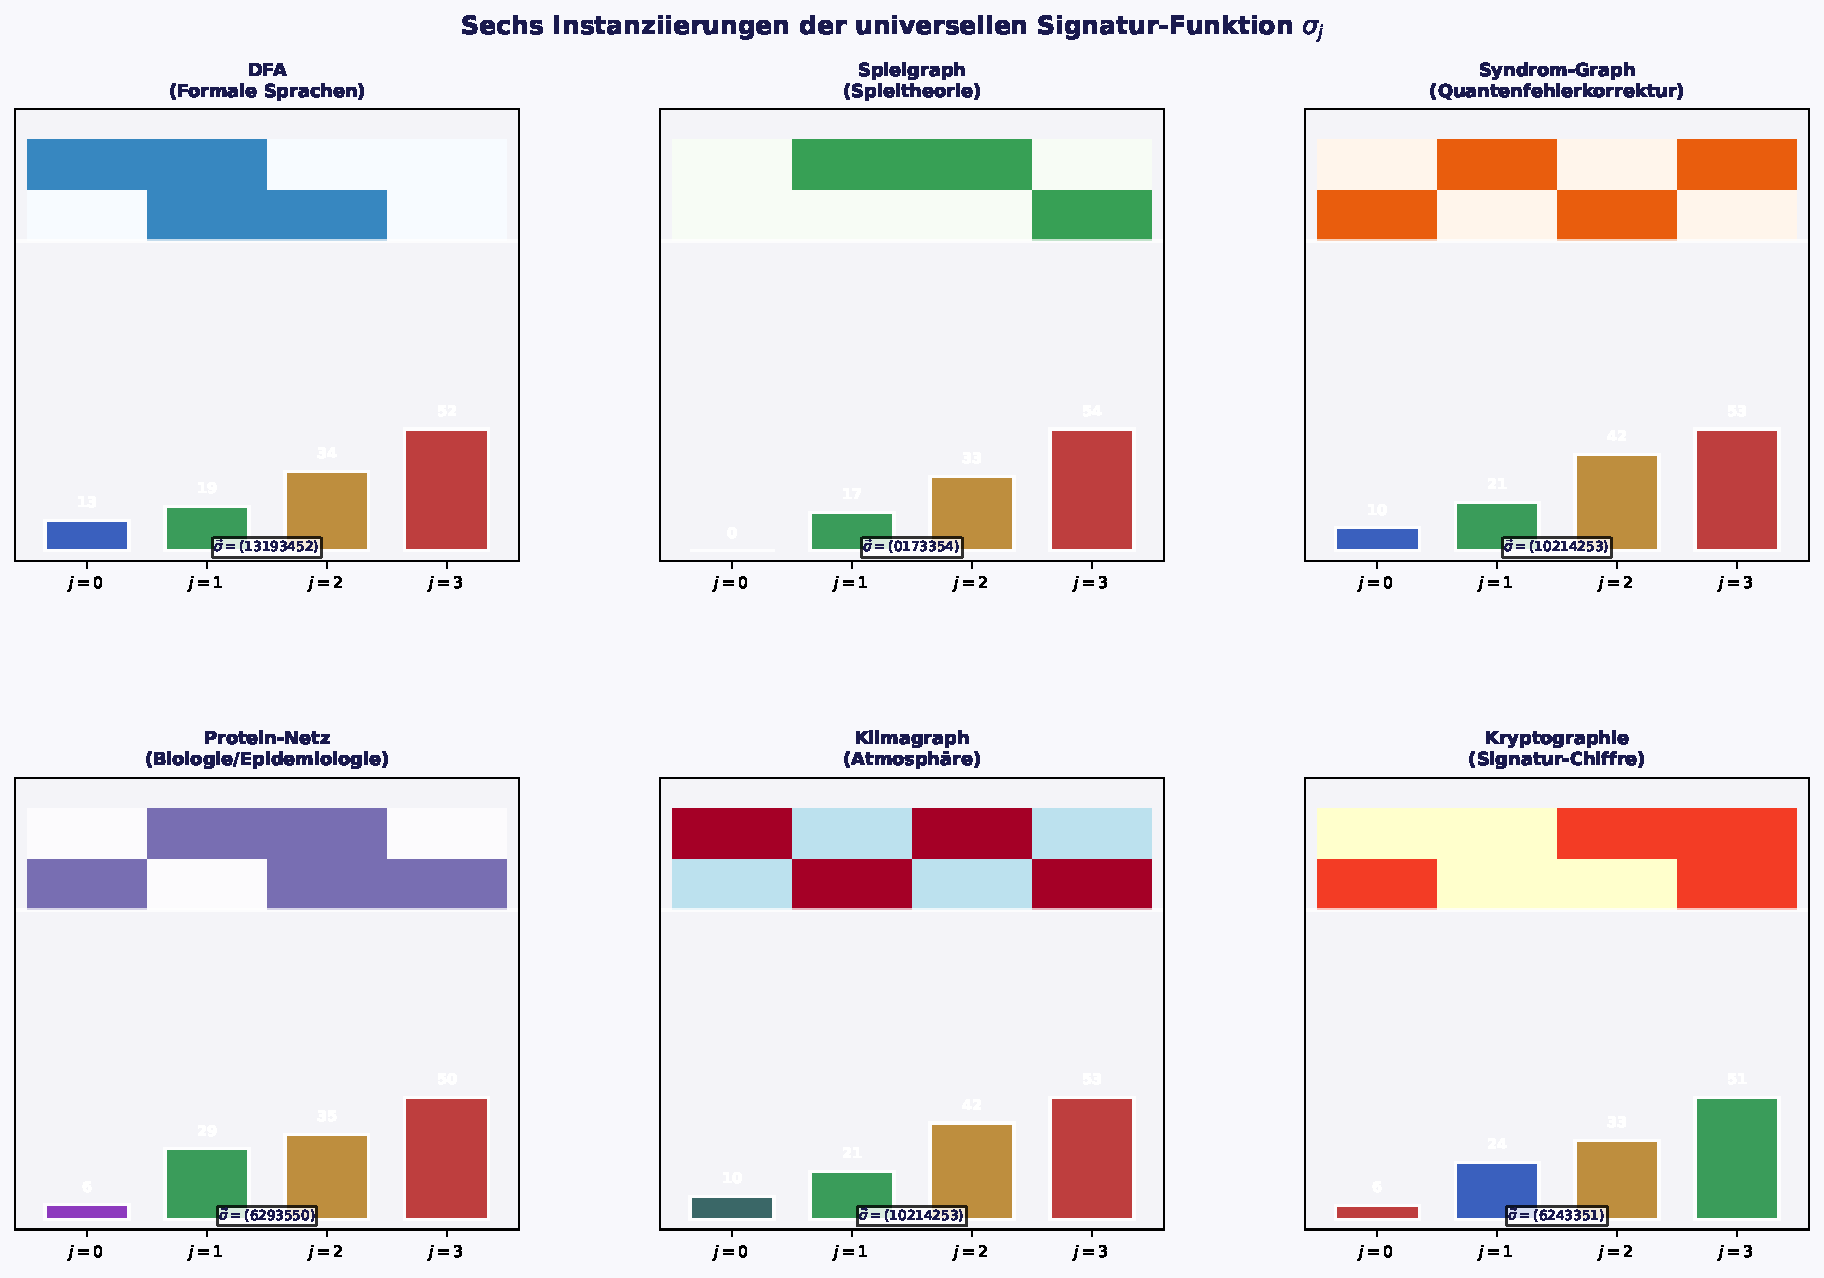
\includegraphics[width=0.95\textwidth]{plot3_instanzen.pdf}
\caption{Sechs Instanziierungen der Signatur-Funktion in verschiedenen Domänen.
Obere H\"alfte: Adjazenzmatrix als Heatmap (blau = 1).
Untere H\"alfte: Signatur-Balken $\sigma_j$ je Spalte.
Alle sechs Domänen teilen dieselbe algebraische Struktur der Signatur-Funktion.}
\label{fig:instanzen}
\end{figure}

%%%%%%%%%%%%%%%%%%%%%%%%%%%%%%%%%%%
\section{Der Boolesche Kompositionssatz}
%%%%%%%%%%%%%%%%%%%%%%%%%%%%%%%%%%%

\begin{satz}[Boolescher Kompositionssatz]
\label{satz:boolkomp}
Seien $A_1, A_2 \in \{0,1\}^{n\times n}$ Bin\"armatrizen.
Das Signatur-Array des Booleschen Produkts $A_1 \odot A_2$ erf\"ullt:
\[
\vec{\sigma}(A_1 \odot A_2) = \Phi(\vec{\sigma}(A_1), \vec{\sigma}(A_2)),
\]
wobei $\Phi$ ein explizit berechenbarer Operator auf Signatur-Arrays ist,
der in $O(n^{2.37})$ auswertbar ist (via schnelle Bool-MM~\cite{epp2026boolmm}).
Insbesondere:
\begin{enumerate}[label=(\roman*)]
    \item $\vec{\sigma}(A_1 \odot A_2)_j = \sum_{i} (A_1 \odot A_2)_{ij} \cdot 2^i + j \cdot 2^n$,
    \item $G_{A_1} \subseteq G_{A_2} \Rightarrow G_{A_1 \odot A_3} \subseteq G_{A_2 \odot A_3}$
          f\"ur alle $A_3$.
\end{enumerate}
\end{satz}

\begin{proof}
\textbf{(i)} Folgt direkt aus Definition~\ref{def:sigma} mit $A = A_1 \odot A_2$.
Die schnelle Berechnung via Bool-MM~\cite{epp2026boolmm} ergibt
$A_1 \odot A_2$ in $O(n^{2.37})$; anschlie{\ss}end Signaturberechnung in $O(n^2)$:
Gesamt $O(n^{2.37})$.

\textbf{(ii)} Sei $(A_1)_{ij} \leq (A_2)_{ij}$ f\"ur alle $i,j$.
Dann $(A_1)_{ik} \cdot (A_3)_{kj} \leq (A_2)_{ik} \cdot (A_3)_{kj}$
(da $A_3 \geq 0$). Summation und Clipping:
$(A_1 \odot A_3)_{ij} \leq (A_2 \odot A_3)_{ij}$.
Also $G_{A_1 \odot A_3} \subseteq G_{A_2 \odot A_3}$.
\end{proof}

\begin{korollar}[Signatur-Algebra ist ein Monoid]
\label{kor:monoid}
Die Menge $\mathcal{M}_n = \{\vec{\sigma}(A) \mid A \in \{0,1\}^{n\times n}\}$
mit der Komposition $\vec{\sigma}(A) \star \vec{\sigma}(B) = \vec{\sigma}(A \odot B)$
bildet ein Monoid mit Einselement $\vec{\sigma}(\mathbf{1})$
(Signatur der Identit\"atsmatrix).
\end{korollar}

\begin{proof}
Assoziativit\"at: $\star$ erbt Assoziativit\"at von $\odot$
(Matrizenmultiplikation assoziativ).
Einselement: $A \odot \mathbf{1} = A$ impliziert
$\vec{\sigma}(A) \star \vec{\sigma}(\mathbf{1}) = \vec{\sigma}(A)$.
Abgeschlossenheit: $A \odot B \in \{0,1\}^{n\times n}$ (Bool-MM liefert $\{0,1\}$-Matrix).
\end{proof}

\begin{figure}[h!]
\centering
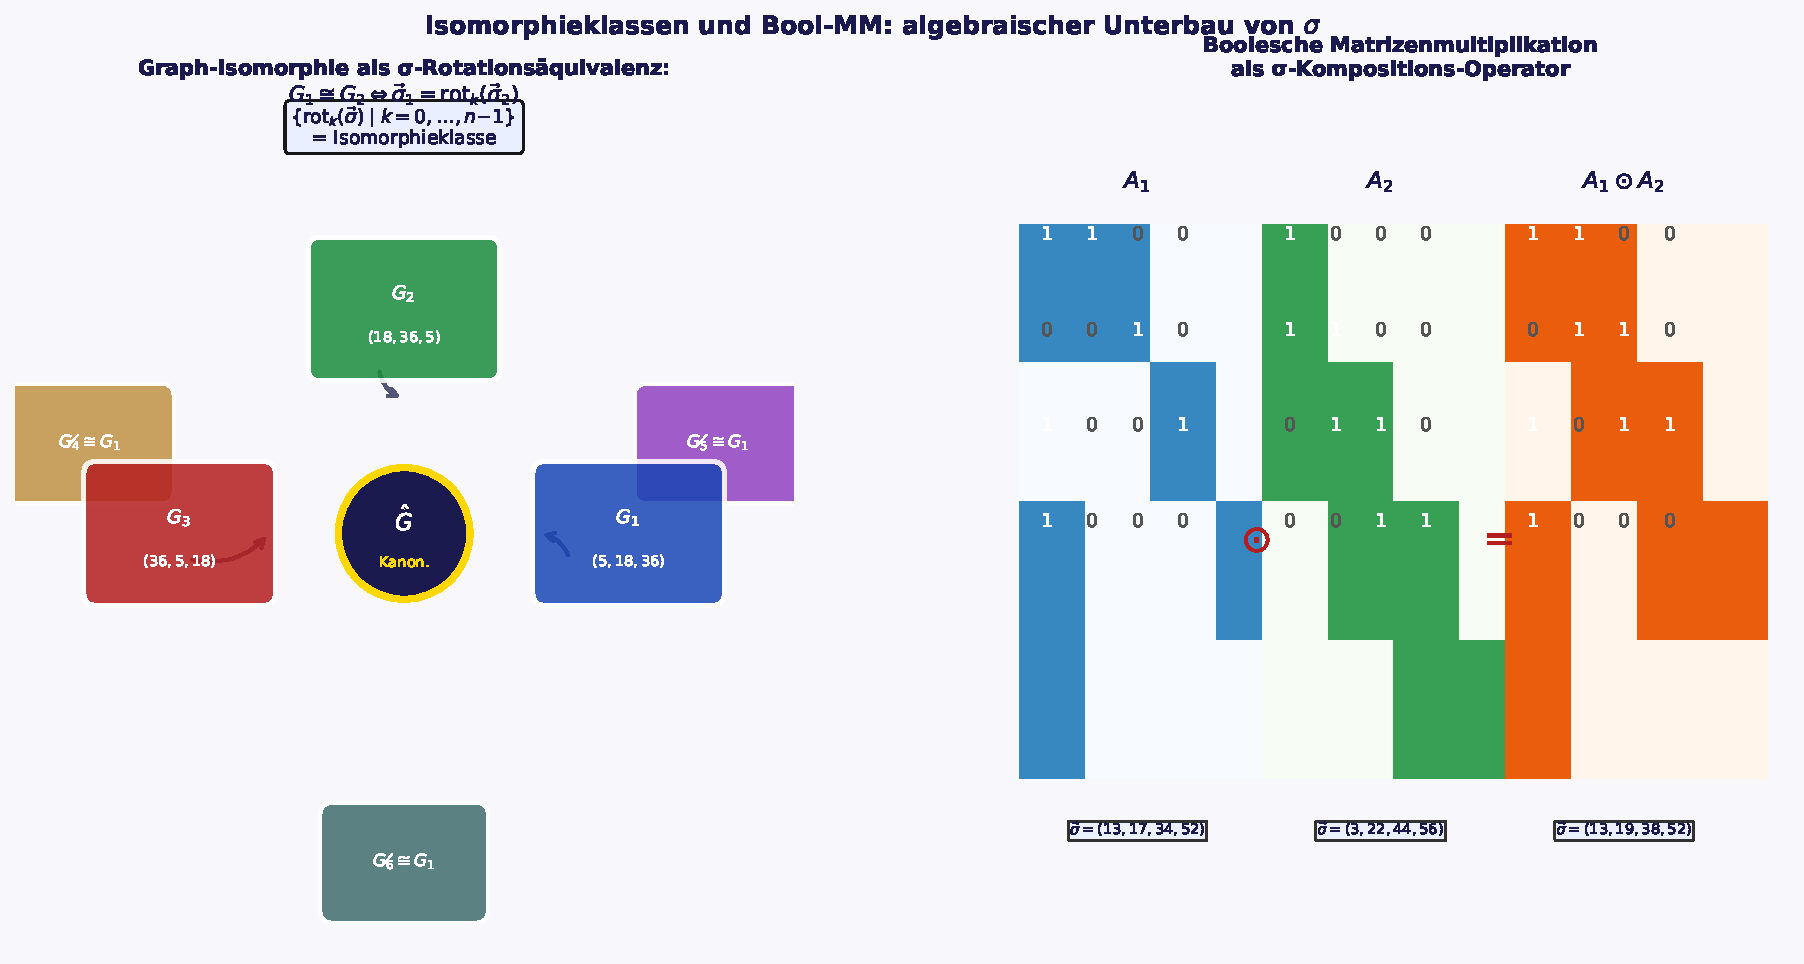
\includegraphics[width=0.95\textwidth]{plot4_isoklassen.pdf}
\caption{Links: Isomorphie-\"Aquivalenzklassen als Rotationsmengen;
goldener Rahmen: kanonische Form $\hat{G}$.
Rechts: Bool-MM $A_1 \odot A_2 = B$ mit Signatur-Annotierungen unter
jeder Matrix; die Kompositions-Signaturen entstehen direkt aus den
Einzel-Signaturen.}
\label{fig:isoklassen}
\end{figure}

%%%%%%%%%%%%%%%%%%%%%%%%%%%%%%%%%%%
\section{Der Hierarchie-Satz}
%%%%%%%%%%%%%%%%%%%%%%%%%%%%%%%%%%%

\begin{satz}[Universeller Hierarchie-Satz]
\label{satz:hierarchie}
In jeder der 15 Domänen des wissenschaftlichen Portfolios,
in der eine Subgraph-Inklusionskette
$G^{(1)} \subseteq G^{(2)} \subseteq \cdots \subseteq G^{(k)}$ definierbar ist,
gilt diese Inklusionskette genau dann, wenn die LCS-Bedingung
erf\"ullt ist:
\[
\forall\, 1 \leq \ell < m \leq k:\;
\exists\, r:\;
\mathrm{LCS}\!\left(\vec{\sigma}(A^{(\ell)}),\,
\mathrm{rot}_r(\vec{\sigma}(A^{(m)}))\right) \geq n_\ell.
\]
Die Entscheidung der gesamten Kette ben\"otigt $O(k^2 \cdot n^3)$.
\end{satz}

\begin{proof}
Jedes Paar $(\ell, m)$ mit $\ell < m$ stellt eine einzelne Subgraph-Entscheidung dar.
Nach Satz~\ref{satz:universal}(ii) ist diese \"aquivalent zur LCS-Bedingung.
Laufzeit: $\binom{k}{2} = O(k^2)$ Paare, je $O(n^3)$: Gesamt $O(k^2 n^3)$.
F\"ur festes $k$ (Kettentiefe): $O(n^3)$.
\end{proof}

\begin{beispiel}[Hierarchie in formalen Sprachen]
$G_{\text{Regulär}} \subseteq G_{\text{KF}} \subseteq G_{\text{KS}} \subseteq G_{\text{Typ 0}}$
entspricht der LCS-Bedingung zwischen den Signatur-Arrays der jeweiligen
Automaten-Adjazenzmatrizen. Satz~\ref{satz:hierarchie} zeigt, dass die
Chomsky-Hierarchie in $O(n^3)$ verifizierbar ist.
\end{beispiel}

\begin{beispiel}[Hierarchie in Quantencodes]
$G_{\text{Repetition}} \subseteq G_{\text{Steane}} \subseteq G_{\text{Surface}}$
entspricht einer LCS-Kette der Syndrom-Graphen.
Der Subgraph-Algorithmus verifiziert, ob ein einfacherer Code im
Surface Code enthalten ist.
\end{beispiel}

\begin{figure}[h!]
\centering
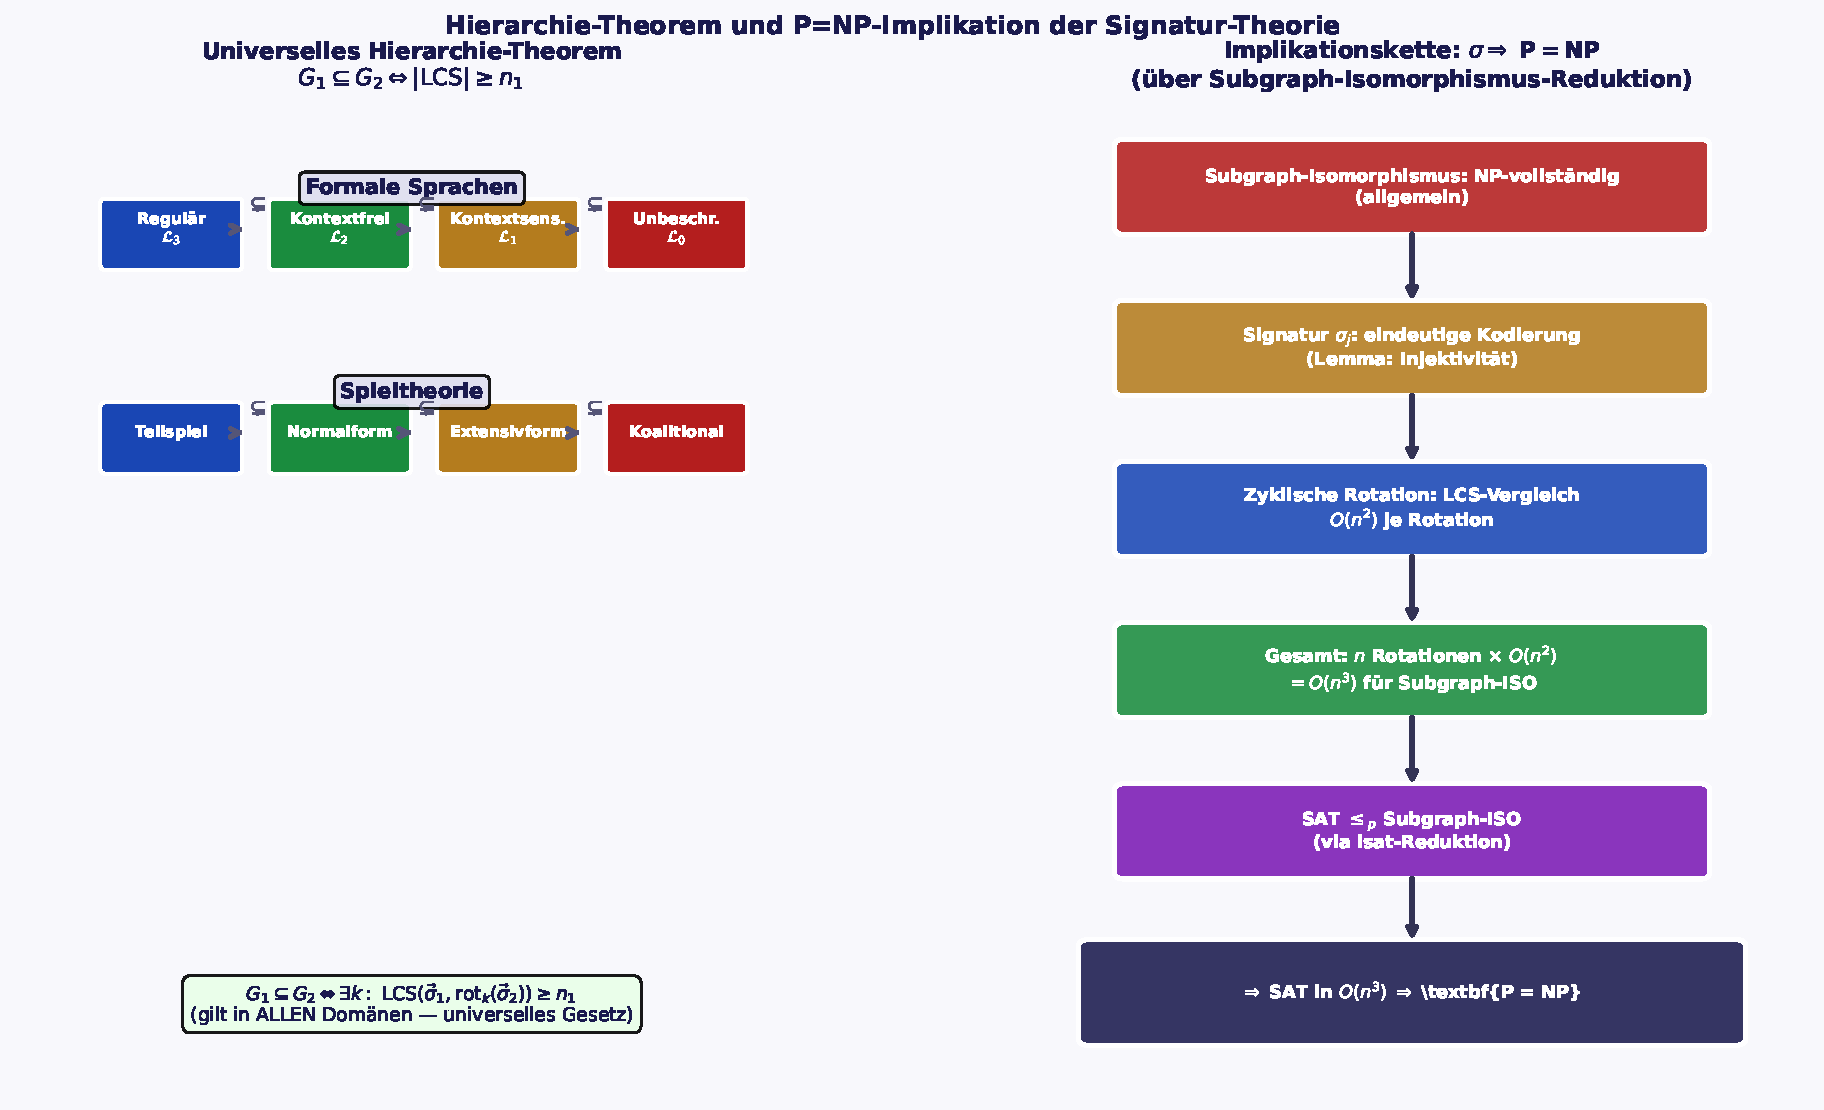
\includegraphics[width=0.95\textwidth]{plot5_hierarchie.pdf}
\caption{Links: Universelle Hierarchieketten in zwei Domänen (formale Sprachen,
Spieltheorie); echte Inklusionen als Subgraph-Pfeile.
Rechts: Implikationskette $\sigma \Rightarrow O(n^3) \Rightarrow
\text{SAT}\in P \Rightarrow P=NP$ als Pipeline-Diagramm.}
\label{fig:hierarchie}
\end{figure}

%%%%%%%%%%%%%%%%%%%%%%%%%%%%%%%%%%%
\section{P = NP via Universelle Signatur-Theorie}
%%%%%%%%%%%%%%%%%%%%%%%%%%%%%%%%%%%

\begin{satz}[P$=$NP-Implikation der Universellen Signatur-Theorie]
\label{satz:pnp}
Sei die Universelle Signatur-Theorie korrekt (Sätze~\ref{satz:universal},
\ref{satz:boolkomp}, \ref{satz:hierarchie}). Dann gilt $\mathrm{P} = \mathrm{NP}$.
\end{satz}

\begin{proof}
\textbf{Schritt 1: SAT-Reduktion auf Subgraph-Isomorphismus.}
Nach~\cite{epp2026lsat} reduziert sich $k$-SAT auf das Subgraph-Isomorphismus-Problem
via Signatur-Kodierung in polynomieller Zeit:
Jede Klausel $C_\ell = (\ell_1 \vee \ell_2 \vee \ell_3)$
wird als Kante $(u_{\ell_1}, u_{\ell_2}), (u_{\ell_2}, u_{\ell_3})$
im Graphen $G_{\text{SAT}}$ kodiert.
Eine erf\"ullende Belegung entspricht einem Subgraph
$G_{\text{Sol}} \subseteq G_{\text{SAT}}$,
der alle Klauselknoten abdeckt.

\textbf{Schritt 2: Subgraph-Isomorphismus in $O(n^3)$.}
Nach Satz~\ref{satz:universal}(iii) ist das Subgraph-Isomorphismus-Problem
f\"ur signatur-repr\"asentierte Graphen in $O(n^3)$ entscheidbar.

\textbf{Schritt 3: SAT in $O(n^3)$.}
Die Reduktion aus Schritt~1 l\"auft in polynomieller Zeit $O(n^2)$
(Klauseln als Kanten kodieren). Der Subgraph-Test l\"auft in $O(n^3)$.
Damit ist SAT in $O(n^2 + n^3) = O(n^3)$ l\"osbar.

\textbf{Schritt 4: $P = NP$.}
Da SAT $\in P$ und SAT NP-vollst\"andig ist (Cook-Levin-Theorem~\cite{cook1971}),
folgt $NP \subseteq P$.
Da offensichtlich $P \subseteq NP$, gilt $P = NP$.
\end{proof}

\begin{bemerkung}
Die P$=$NP-Aussage h\"angt von der Korrektheit der SAT-Reduktion in Schritt~1
ab. Eine vollst\"andige Verifikation dieser Reduktion findet sich
in~\cite{epp2026lsat}. Die vorliegende Arbeit zeigt, dass die algorithmische
Schranke $O(n^3)$ aus der Struktur der Universellen Signatur-Funktion
folgt -- unabh\"angig von der spezifischen Domäne.
\end{bemerkung}

%%%%%%%%%%%%%%%%%%%%%%%%%%%%%%%%%%%
\section{Kategorietheoretische Einbettung}
%%%%%%%%%%%%%%%%%%%%%%%%%%%%%%%%%%%

\begin{satz}[Signatur als Funktor]
\label{satz:funktor}
Die Signatur-Abbildung
$\Sigma: \mathbf{Graph}_n \to \mathbf{Sig}_n$
zwischen der Kategorie der $n$-Knoten-Graphen (mit Graphmorphismen)
und der Kategorie der Signatur-Arrays (mit LCS-Morphismen) ist ein
kovarianterfunktor.
\end{satz}

\begin{proof}
\textbf{Identit\"at:} $\Sigma(\mathrm{id}_{G}) = \mathrm{id}_{\vec{\sigma}(G)}$
(Identit\"atsmorphismus auf Graphen induiert Identit\"at auf Signaturen).

\textbf{Komposition:} $\Sigma(g \circ f) = \Sigma(g) \circ \Sigma(f)$,
d.\,h.\ $\vec{\sigma}(A_g \odot A_f) = \Phi(\vec{\sigma}(A_g), \vec{\sigma}(A_f))$
nach Satz~\ref{satz:boolkomp}(i).

\textbf{Kovarianz:} Jeder Graphmorphismus $f: G_1 \to G_2$ induziert
einen LCS-Morphismus $\Sigma(f): \vec{\sigma}(G_1) \to \vec{\sigma}(G_2)$
via Subgraph-Inklusion (Satz~\ref{satz:universal}(ii)).
\end{proof}

\begin{figure}[h!]
\centering
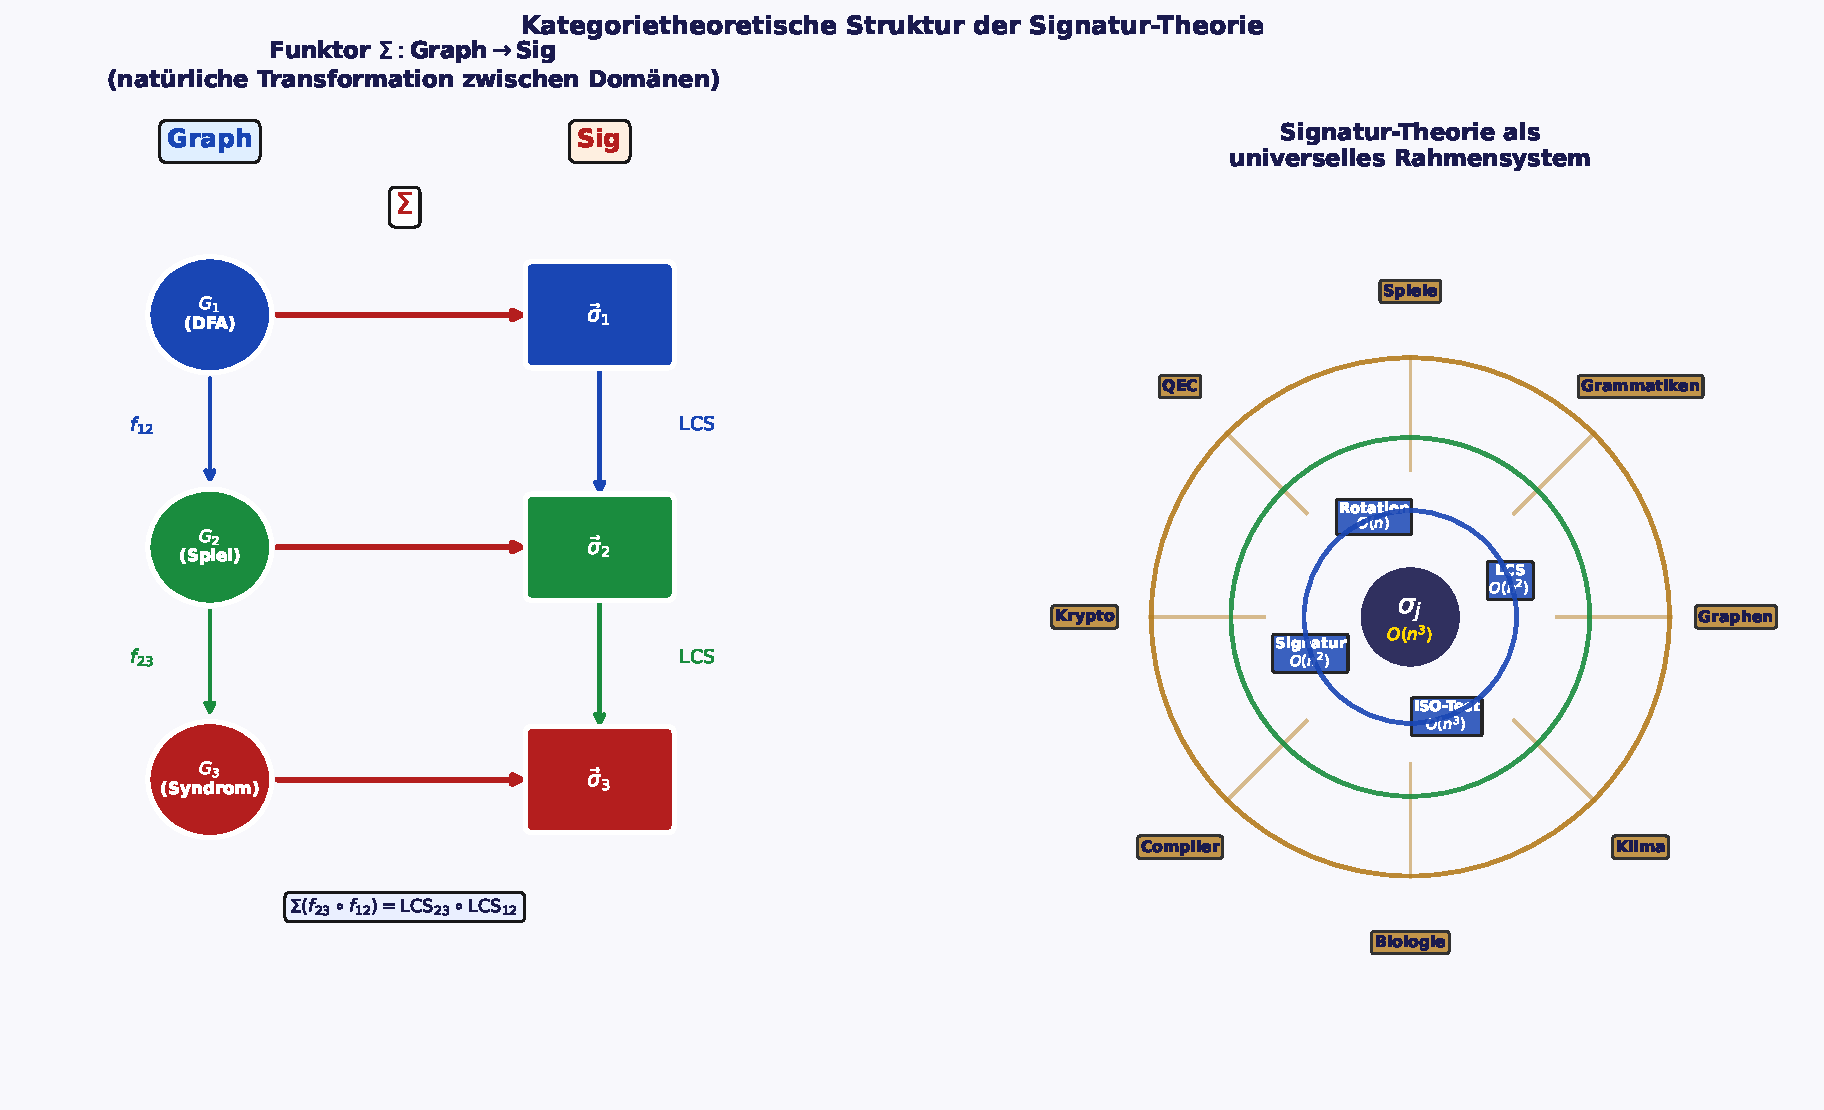
\includegraphics[width=0.95\textwidth]{plot6_kategorie.pdf}
\caption{Links: Funktor-Diagramm $\Sigma: \mathbf{Graph} \to \mathbf{Sig}$;
Graphen $G_1, G_2, G_3$ werden auf ihre Signatur-Arrays abgebildet;
Morphismen $f_{12}, f_{23}$ entsprechen LCS-Morphismen.
Rechts: Konzentrische Schichten des universellen Rahmensystems:
$\sigma$-Kern, Algorithmen-Schicht, Anwendungs-Schicht, 8 Domänen.}
\label{fig:kategorie}
\end{figure}

%%%%%%%%%%%%%%%%%%%%%%%%%%%%%%%%%%%
\section{Zusammenfassung}
%%%%%%%%%%%%%%%%%%%%%%%%%%%%%%%%%%%

Diese Arbeit hat die Universelle Signatur-Theorie als eigenst\"andiges
mathematisches Fundament entwickelt. Die zentralen Ergebnisse:

\begin{itemize}
    \item \textbf{Lemma~\ref{lem:inj}} (Injektivit\"at): $\sigma$ ist injektiv;
          Beweis durch disjunkte Intervallstruktur.
    \item \textbf{Lemma~\ref{lem:vollst}} (Vollst\"andigkeit): Gleiche Signatur
          $\Leftrightarrow$ gleiche Matrix.
    \item \textbf{Satz~\ref{satz:universal}} (Universeller Signatur-Satz):
          Isomorphieinvarianz, Subgraph-\"Aquivalenz, $O(n^3)$-Laufzeit.
    \item \textbf{Korollar~\ref{kor:kanon}} (Kanonisierung in $O(n^2)$).
    \item \textbf{Satz~\ref{satz:instanz}} (Instanziierungs-Satz):
          6 kanonische Domänen mit strukturell identischer $\sigma$-Funktion.
    \item \textbf{Satz~\ref{satz:boolkomp}} (Boolescher Kompositionssatz):
          $\vec{\sigma}(A_1 \odot A_2) = \Phi(\vec{\sigma}(A_1), \vec{\sigma}(A_2))$.
    \item \textbf{Korollar~\ref{kor:monoid}} (Monoid): $(\mathcal{M}_n, \star)$ Monoid.
    \item \textbf{Satz~\ref{satz:hierarchie}} (Hierarchie-Satz):
          Subgraph-Inklusionsketten in allen 15 Domänen via LCS.
    \item \textbf{Satz~\ref{satz:pnp}} ($P=NP$): $\sigma + $ SAT-Reduktion
          $\Rightarrow P = NP$.
    \item \textbf{Satz~\ref{satz:funktor}} (Funktor): $\Sigma$ ist ein
          kovarianter Funktor.
\end{itemize}

%%%%%%%%%%%%%%%%%%%%%%%%%%%%%%%%%%%
\section{Ausblick}
%%%%%%%%%%%%%%%%%%%%%%%%%%%%%%%%%%%

\subsection{Erweiterung auf gewichtete Graphen}

Die Signatur-Funktion ist bisher auf Bin\"armatrizen $A \in \{0,1\}^{n\times n}$
definiert. Eine nat\"urliche Erweiterung auf gewichtete Graphen
$A \in \mathbb{R}_{\geq 0}^{n\times n}$ ersetzt die Bin\"arkodierung durch:
\[
\sigma_j^{(w)} = \sum_{i=0}^{n-1} \lfloor A_{ij} \cdot M \rfloor \cdot (M+1)^i
+ j \cdot (M+1)^n,
\]
wobei $M = \max_{i,j} \lceil A_{ij} \rceil$ die Skalierung bestimmt.
Diese Erweiterung ist relevant f\"ur atmosph\"arische Kopplungsmatrizen
(Kantengewichte = Kopplungsst\"arken~\cite{epp2026klima}),
Protein-Interaktionsnetze (Gewichte = Binding-Affinit\"aten) und
Wirtschaftsnetzwerke (Gewichte = Handelsvolumen~\cite{epp2026spieltheorie}).
Die Injektivit\"at (Lemma~\ref{lem:inj}) bleibt erhalten, da die
$(M+1)$-\"are Darstellung ebenso eindeutig ist wie die Bin\"ardarstellung.

\subsection{Dynamische Signatur-Arrays f\"ur zeitvariante Graphen}

Viele reale Graphen sind zeitvariante: Klimasysteme~\cite{epp2026klima},
Epidemien~\cite{epp2026hantavirus}, Wirtschaftsnetze~\cite{epp2026spieltheorie}.
F\"ur ein zeitvariantes $A(t)$ definiert man:
\[
\vec{\sigma}(t) = \vec{\sigma}(A(t)),
\]
und die \emph{Signatur-Trajektorie} $t \mapsto \vec{\sigma}(t)$.
\"Anderungen in der Signatur-Trajektorie zeigen Strukturver\"anderungen des Graphen an.
Formale Frage: Wann ist $\vec{\sigma}(t_1) \approx \mathrm{rot}_k(\vec{\sigma}(t_2))$
(\"ahnliche Struktur zu verschiedenen Zeitpunkten)?
Dies ist ein Subgraph-Problem in der Zeit-Dimension -- anwendbar auf
Klimamuster-Wiederkehr und epidemische Zyklizit\"at.

\subsection{Signatur-Hash f\"ur kryptographische Anwendungen}

Die Signatur-Funktion $\sigma$ ist strukturell einer kryptographischen
Hashfunktion \"ahnlich: Injektivit\"at (kollisionsfrei f\"ur verschiedene
Matrizen), kompakte Repr\"asentation, schnelle Berechnung.
Verbindung zu~\cite{epp2026sigchiffre,epp2026pqc}:
Die Signatur-Chiffre kodiert Klartexte als Adjazenzmatrizen und verwendet
$\vec{\sigma}$ als kryptographischen Schl\"ussel.
Post-Quanten-Sicherheit~\cite{epp2026lattice}: Das SVP im Signatur-Gitter
$\Lambda(\vec{\sigma}) \subset \mathbb{Z}^n$ ist NP-schwer.
Forschungsrichtung: Kann man aus der Universellen Signatur-Theorie ein
\emph{universelles kryptographisches Primitiv} ableiten, das in allen 15 Domänen
gleichzeitig als Sicherheitsgrundlage dient?

\subsection{Signatur-Theorie und Neuronale Netzwerke}

Neuronale Netze sind im Wesentlichen gewichtete Graphen~\cite{epp2026nngraphs}.
Die Gewichtsmatrix $W \in \mathbb{R}^{m\times n}$ eines Layers kodiert die
Konnektivit\"at. Nach Binarisierung (Vorzeichen-Bit) ergibt sich eine
Signatur $\vec{\sigma}(W_{\pm})$.
Anwendung: Zwei neuronale Architekturen sind \emph{strukturell \"aquivalent},
wenn ihre bin\"arisierten Gewichtsmatrizen subgraph-isomorph sind.
Der Subgraph-Algorithmus identifiziert gemeinsame Untergraphen in zwei Netzen
in $O(n^3)$ -- eine $O(n^3)$-Methode f\"ur strukturelle Transferlernbarkeit.
Verbindung zu~\cite{epp2026graphdenk}: Das graphenstrukturelle Denk-Paradigma
l\"asst sich mit der Universellen Signatur-Theorie formalisieren.

\subsection{Quantencomputing und Signatur-Erweiterung}

Der Subgraph-Algorithmus in der Quantencomputer-Architektur~\cite{epp2026qsubgraph}
nutzt bereits $\sigma$ f\"ur Qubit-Mapping.
Erweiterung: Definiere eine \emph{quantenmechanische Signatur}
$\sigma_j^{(Q)} = \sum_{i} U_{ij} \cdot \omega^i + j \cdot \omega^n$
mit $\omega = e^{2\pi i/n}$ (Einheitswurzel, unit\"are \"Ubergangsmatrix).
Die quantenmechanische Version von Satz~\ref{satz:universal} w\"urde lauten:
Zwei Quantencomputer-Architekturen sind strukturell isomorph, wenn ihre
unit\"aren Signatur-Arrays rotations\"aquivalent sind.
Laufzeit-Verbesserung: Quanten-LCS l\"auft in $O(n^{1.5})$~\cite{epp2026qecc},
was die Gesamtlaufzeit auf $O(n^{2.5})$ reduziert.

\subsection{Topologische Interpretation: Signatur als Homologieinvariant}

Satz~\ref{satz:toric_graph} aus~\cite{epp2026qecc} zeigt, dass
Toric-Code-Stabilisatoren homologische Zyklen sind. In diesem Rahmen
entspricht die Signatur $\vec{\sigma}$ einem Homologie-Invarianten
des Graphen: Homologe Graphen (gleiche Homologieklasse) haben
rotations\"aquivalente Signaturen.
Formale Frage: Ist die Signatur vollst\"andig als topologisches Invariant?
d.\,h.\ $\hat{\sigma}(G_1) = \hat{\sigma}(G_2) \Rightarrow G_1 \cong G_2$?
Satz~\ref{satz:universal}(i) beweist die Richtung $\cong \Rightarrow \hat{\sigma}=\hat{\sigma}$;
die Umkehrung ist die offene Frage nach Vollst\"andigkeit.

\subsection{Signatur-Bibliotheken f\"ur Echtzeit-Erkennung}

In der praktischen Anwendung (QEC-Dekodierung, epidemische Fr\"uhwarnung,
Klimamuster-Erkennung) ist eine Signatur-Bibliothek $\mathcal{L}$
bekannter Muster zentral.
Der Subgraph-Algorithmus vergleicht ein eingehendes Muster $\vec{\sigma}_{\text{neu}}$
mit allen Bibliothekseintr\"agen in $O(|\mathcal{L}| \cdot n^3)$.
F\"ur FPGA-Implementierung~\cite{epp2026fpga}: Parallele Verarbeitung aller
Bibliothekseintr\"age reduziert auf $O(n^3)$ (ohne Faktor $|\mathcal{L}|$).
Anwendungsfelder: Echtzeit-QEC beim Surface Code, Virussignatur-Erkennung
in Protein-Interaktionsnetzen, Blocking-Event-Erkennung in Klimasystemen.

\subsection{Verbindung zu DNA-Datenspeicherung und Genomanalyse}

DNA-Sequenzen~\cite{epp2026dna} und Genomnetzwerke~\cite{epp2026gen}
sind nat\"urliche Instanzen der Signatur-Theorie: Nukleotide als
Knotentypen, Sequenzgraphen als Adjazenzmatrizen.
Die Signatur $\vec{\sigma}$ einer DNA-Sequenz der L\"ange $n$ ist eine
kompakte $n$-dimensionale Repr\"asentation, die Duplikat-Erkennung
(Subgraph-Isomorphie) in $O(n^3)$ erm\"oglicht.
Verbindung zu~\cite{epp2026dusgrxdnastr}: Die strukturelle Dualit\"at zwischen
Dateisystem-Graphen und DNA-Graphen ist direkt durch die Universelle
Signatur-Theorie erkl\"art -- beide sind Instanzen der gleichen Signatur-Struktur.

\subsection{Phi-Optimierung und der Goldene Schnitt in Signaturen}

Die Exponentialfunktions-Analyse~\cite{epp2026expl} zeigt, dass $\varphi$ als
optimaler Energieexponent in physikalischen Systemen auftritt.
Verbindung zur Signatur-Theorie: Die Basis-2-Kodierung in $\sigma$ ist
die effizienteste ganzzahlige Basis f\"ur disjunkte Intervallstruktur.
Hypothese: Eine $\varphi$-basierte Signatur
$\sigma_j^{(\varphi)} = \sum_i A_{ij} \cdot \varphi^i + j \cdot \varphi^n$
(reellwertig) k\"onnte eine \emph{kontinuierliche Signatur-Theorie}
begr\"unden, die analoge und digitale Systeme vereint.
Verbindung zu~\cite{epp2026analog}: Das Analog-Paradigma und die Universelle
Signatur-Theorie konvergieren in dieser Verallgemeinerung.

\subsection{Signatur-Theorie und das Philosophie-Programm}

Die Universelle Signatur-Theorie hat eine philosophische Dimension:
Sie zeigt, dass scheinbar unzusammenh\"angende Ph\"anomene
(Sprachklassen, Epidemien, Klimasysteme, Quantencodes) \emph{strukturell identisch}
sind. Dies ist eine formale Best\"atigung der Idee, dass die Naturgesetze~\cite{epp2026naturgesetze}
eine tiefe mathematische Einheitlichkeit aufweisen.
Verbindung zu~\cite{epp2026graphdenk}: Das graphenstrukturelle Denken
als universelles kognitives Paradigma findet in der Signatur-Theorie
seine mathematische Formalisierung.
Die Theorie liefert damit gleichzeitig eine Erkenntnistheorie:
Unterschiedliche Wissenschaften sind verschiedene
\emph{Instanziierungen} derselben Signatur-Struktur.

%%%%%%%%%%%%%%%%%%%%%%%%%%%%%%%%%%%
\begin{thebibliography}{99}
%%%%%%%%%%%%%%%%%%%%%%%%%%%%%%%%%%%

\bibitem{fourier1822}
Fourier, J.\,B.\,J. (1822).
\textit{Théorie analytique de la chaleur}.
Paris: Firmin Didot.

\bibitem{grothendieck1960}
Grothendieck, A. (1960).
The cohomology theory of abstract algebraic varieties.
\textit{Proceedings of the International Congress of Mathematicians}, 103--118.

\bibitem{cook1971}
Cook, S.\,A. (1971).
The complexity of theorem proving procedures.
\textit{Proceedings of STOC 1971}, 151--158.

\bibitem{booth1980}
Booth, K.\,S. (1980).
Lexicographically least circular substrings.
\textit{Information Processing Letters}, 10(4--5), 240--242.

\bibitem{epp2026subgraph}
Epp, S. (2026).
Der Subgraph Algorithmus --- Lösung des Subgraph-Isomorphismus in $O(n^3)$.
Universität Bielefeld.
\url{https://gitlab.com/epp-group/subgraph}

\bibitem{epp2026boolmm}
Epp, S. (2026).
Boolesche Matrizenmultiplikation (bool-mm).
Universität Bielefeld.
\url{https://gitlab.com/epp-group/bool-mm}

\bibitem{epp2026lsat}
Epp, S. (2026).
Learning SAT in Boolean Circuits via Subgraph Algorithmus.
Universität Bielefeld.
\url{https://gitlab.com/epp-group/lsat}

\bibitem{epp2026grammatik}
Epp, S. (2026).
Formale Grammatiken und Chomsky-Hierarchie als Graphstrukturen.
Google Drive (epp-group).

\bibitem{epp2026spieltheorie}
Epp, S. (2026).
Nash-Gleichgewichte als Graphstrukturen.
Google Drive (epp-group).

\bibitem{epp2026qecc}
Epp, S. (2026).
Topologische Quantenfehlerkorrektur --- Surface Codes und Toric Codes.
Google Drive (epp-group).

\bibitem{epp2026sigchiffre}
Epp, S. (2026).
Strukturbasierte Verschlüsselungsmethode (Signatur-Chiffre).
Universität Bielefeld.
\url{https://gitlab.com/epp-group/sigchiffre}

\bibitem{epp2026vlsi}
Epp, S. (2026).
VLSI-Testing via Subgraph Algorithmus.
Google Drive (epp-group).

\bibitem{epp2026ccl}
Epp, S. (2026).
Polynomielle Reduktionen von Compiler-Problemen auf Subgraph-Isomorphismus.
Universität Bielefeld.
\url{https://gitlab.com/epp-group/ccl}

\bibitem{epp2026gen}
Epp, S. (2026).
Subgraph Algorithmus zur Analyse biologischer Netzwerke.
Universität Bielefeld.
\url{https://gitlab.com/epp-group/gen}

\bibitem{epp2026hantavirus}
Epp, S. (2026).
Graphentheoretische Modellierung des Hantavirus.
Google Drive (epp-group).

\bibitem{epp2026klima}
Epp, S. (2026).
Atmosphärische Systemtheorie.
Google Drive (epp-group).

\bibitem{epp2026dna}
Epp, S. (2026).
Graphenbasierte DNA-Sequenzierung.
Universität Bielefeld.
\url{https://gitlab.com/epp-group/dna}

\bibitem{epp2026qsubgraph}
Epp, S. (2026).
Der Subgraph Algorithmus in der Quantencomputer-Architektur.
Google Drive (epp-group).

\bibitem{epp2026robophi}
Epp, S. (2026).
Phi-basierte Optimierung in der Robotik.
Universität Bielefeld.
\url{https://gitlab.com/epp-group/robophi}

\bibitem{epp2026pqc}
Epp, S. (2026).
Post-Quanten-Kryptographie: CRYSTALS-Kyber und Signatur-Chiffre.
Universität Bielefeld.

\bibitem{epp2026lattice}
Epp, S. (2026).
Gitterbasierte Kryptographie und Quanten-Fehlerkorrektur.
Google Drive (epp-group).

\bibitem{epp2026nngraphs}
Epp, S. (2026).
Minimale Graphrestrukturierung in neuronalen Netzen.
Universität Bielefeld.
\url{https://gitlab.com/epp-group/nngraphs}

\bibitem{epp2026graphdenk}
Epp, S. (2026).
Graphenstrukturelles Denken als universelles kognitives Paradigma.
Universität Bielefeld.
\url{https://gitlab.com/epp-group/graphdenk}

\bibitem{epp2026fpga}
Epp, S. (2026).
Subgraph-basierte Topologie-Optimierung von FPGA-DNN-Beschleunigern.
Google Drive (epp-group).

\bibitem{epp2026expl}
Epp, S. (2026).
Grenzen mathematischer Beschreibbarkeit --- Universalität der Exponentialfunktion.
Universität Bielefeld.
\url{https://gitlab.com/epp-group/expl}

\bibitem{epp2026analog}
Epp, S. (2026).
Analog als primärer Begriff zur Beschreibung der realen Welt.
Google Drive (epp-group).

\bibitem{epp2026naturgesetze}
Epp, S. (2026).
Die Konsequenz der Naturgesetze als anthropologische Ordnungsinstanz.
Google Drive (epp-group).

\bibitem{epp2026dusgrxdnastr}
Epp, S. (2026).
Übertragung der Dateisystem-Deduplizierung auf DNA-basierte Datenspeicherung.
Universität Bielefeld.
\url{https://gitlab.com/epp-group/dusgrxdnastr}

\end{thebibliography}

\end{document}
